\section{Applications}
    %%%%%%%%%%%%%%%%%%%%%%%%%%%%%%%%%%%%%%%%
    %%  Slide 1: <Applications>  %%
    %%%%%%%%%%%%%%%%%%%%%%%%%%%%%%%%%%%%%%%%
    \begin{frame}
        \frametitle{Applications}
        \textbf{Tracking in HEP experiments:} 
        \begin{itemize}
            \item pattern recognition with the identification of particle tracks even in the presence of large backgrounds and pile-up
            \item measurement of vertices (primary and secondary)
            \item multi-track and vertex separation in the core of jets
            \item measurement of specific ionization
            \item momentum measurement combining with the information from other detectors
        \end{itemize}
        Many developments whose main promoters are ALICE (ALPIDE sensor and thinning), ATLAS ITK (study on the Monopix series and on MALTA) and Belle2.\\
        \medskip
        But also \textbf{other} possible applications as in space-experiments and in medicine (dosimetry? Later in the presentation). 

    \end{frame} 


    %%%%%%%%%%%%%%%%%%%%%%%%%%%%%%%%%%%%%%%%
    %%  Slide 1: <ALICE>  %%
    %%%%%%%%%%%%%%%%%%%%%%%%%%%%%%%%%%%%%%%%
    \begin{frame}
        \frametitle{ALPIDE - ALice PIxel DEtector}
        \begin{columns}
            \column{0.5\textwidth}  
                \centering
                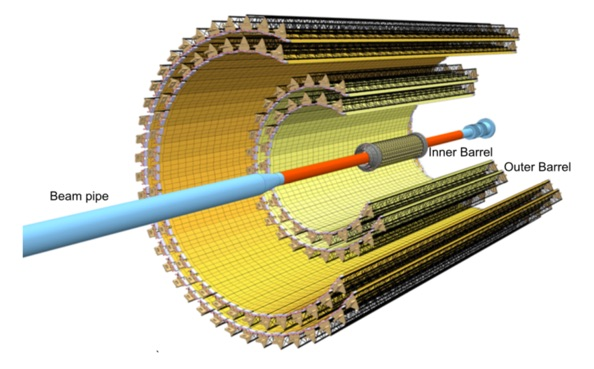
\includegraphics[width=.99\linewidth]{figures/pixel_detectors_usage/alice.png}
            \column{0.5\textwidth}
            ALICE ITS2 upgraded in 2019-20\\
            \smallskip
            The \textbf{sensor} uses high resistivity p-type epi-layer, TowerJazz in \SI{0.18}{\um}. It is the first large area $\sim$\SI{10}{m\squared} MAPS detector with sparsified readout.

        \end{columns}
        \begin{itemize}
            \item position measurement $\sim$\SI{5}{\um} (pixel dimension 27$\times$29\si{\um\squared})
            \item X$_0$ reduced from 1.14\% to 0.3\% per layer
            \item efficiency of track reconstruction improves of a factor 6 for low momentum particles with $p_T \sim$\SI{0.1}{GeV/c}
        \end{itemize}
        \medskip
         
        ALPIDE is under test for several other HEP detectors (i.e. Belle2) and applications and many MAPS have an ALPIDE-based front end (i.e. TJ-Monopix1, ARCADIA)

    \end{frame} 

    
    %%%%%%%%%%%%%%%%%%%%%%%%%%%%%%%%%%%%%%%%
    %%  Slide 1: <>  %%
    %%%%%%%%%%%%%%%%%%%%%%%%%%%%%%%%%%%%%%%%
    \begin{frame}
        \frametitle{Applicability in FLASH radiotherapy}
        Radiotherapy uses the damage causes by the ionization of energy loss by particles. FLASH-RT consists of delivering the dose in a small fraction of time. FLASH-RT reduces the toxiticy of the radiation on healty tissues
        \begin{columns}
            \column{0.6\textwidth}  
                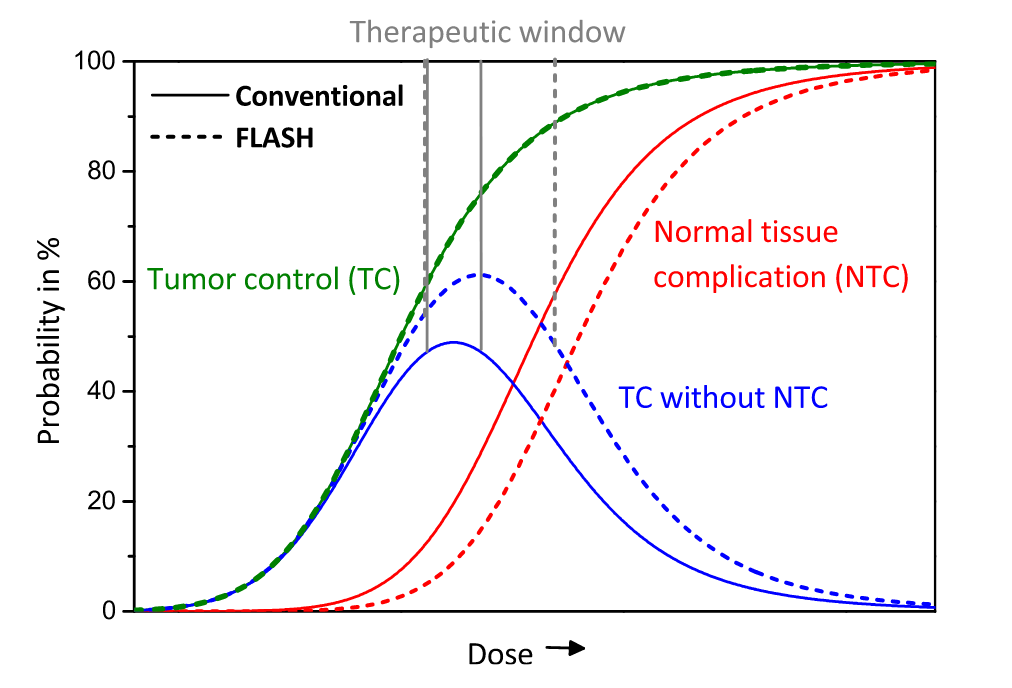
\includegraphics[width=.99\linewidth]{figures/pixel_detectors_usage/curve_flash.png}
        \column{0.6\textwidth} 
            
            \begin{table}
                \tiny
                \begin{center}
                \begin{tabular}{|c | c |c |}
                \hline
                & CONV-RT & FLASH-RT \\
                \hline
                \hline
                Dose rate & \SI{0.03}{Gy/s} & \SI{40}{Gy/s}\\
                Intra pulse dose rate & \SI{100}{Gy/s}&\SI{10 6}{Gy/s}\\
                Treatment duration & $\sim$minutes & $\lessapprox$\SI{500}{ms} \\
                Dose Per Pulse & \SI{0.3}{mGy} & 1-10 Gy\\
                Pulse width & \SI{3}{\us} & $\sim$\SI{2}{\us} \\
                \hline
                \end{tabular}
                \end{center}
            \end{table}        
        \end{columns}
    \end{frame} 



    %%%%%%%%%%%%%%%%%%%%%%%%%%%%%%%%%%%%%%%%
    %%  Slide 1: <dosimeters>  %%
    %%%%%%%%%%%%%%%%%%%%%%%%%%%%%%%%%%%%%%%%
    \begin{frame}
        \frametitle{FLASH-RT}
        \begin{itemize}
            \item new dosimeters need to be tissue equivalent 
            \item beam monitor
            \item diagnostics
        \end{itemize}
        Different charateristics, and different requirement. 
        All online detector types show saturation problems at high intensity.


    \end{frame}     